%%%%%%%%%%%%%%%%%%%%%%%%%%%%%%%%%%%%%%%%%%%%%%%%%%%%%%%%%%%%%%%%%%%%%
%
% CS484 Written Question Template
%
% This is a LaTeX document. LaTeX is a markup language for producing 
% documents. Your task is to fill out this document, then to compile 
% it into a PDF document. 
%
% 
% TO COMPILE:
% > pdflatex thisfile.tex
%
% If you do not have LaTeX and need a LaTeX distribution:
% - Personal laptops (all common OS): www.latex-project.org/get/
% - We recommend miktex (https://miktex.org/) for latex engine,
%   and TeXstudio(http://www.texstudio.org/) for latex editor.
%   You should install both programs for editing latex.
%   Or you can use Overleaf (https://www.overleaf.com/) which is 
%   an online latex editor.
%
% If you need help with LaTeX, please come to office hours. 
% Or, there is plenty of help online:
% https://en.wikibooks.org/wiki/LaTeX
%
% Good luck!
% Min and the CS484 staff
%
%%%%%%%%%%%%%%%%%%%%%%%%%%%%%%%%%%%%%%%%%%%%%%%%%%%%%%%%%%%%%%%%%%%%%

\documentclass[11pt]{article}

\usepackage[english]{babel}
\usepackage[utf8]{inputenc}
\usepackage[colorlinks = true,
			linkcolor = blue,
			urlcolor  = blue]{hyperref}
\usepackage[a4paper,margin=1.5in]{geometry}
\usepackage{stackengine,graphicx}
\usepackage{fancyhdr}
\setlength{\headheight}{15pt}
\usepackage{microtype}
\usepackage{times}
\usepackage{booktabs}
\usepackage{listings}
\usepackage{xcolor}
\lstdefinestyle{codestyle}{
	frame=single,
	basicstyle=\ttfamily\footnotesize,
	keywordstyle=\bfseries\color{magenta},
	commentstyle=\itshape\color{gray},
	stringstyle=\color{orange},
	numberstyle=\sffamily\scriptsize\color{gray},
	showspaces=false,
	showstringspaces=false,
	showtabs=false,
	tabsize=4,
	breakatwhitespace=false,
	breaklines=true,
	keepspaces=true,
	captionpos=b,
	numbers=left,
	numbersep=5pt}
\lstset{style=codestyle}

\frenchspacing
\setlength{\parindent}{0cm} % Default is 15pt.
\setlength{\parskip}{0.3cm plus1mm minus1mm}

\pagestyle{fancy}
\fancyhf{}
\lhead{Homework 1 Questions}
\rhead{CS484}
\rfoot{\thepage}

\date{}

\title{\vspace{-1cm}Homework 1 Questions}


\begin{document}
\maketitle
\vspace{-2cm}
\thispagestyle{fancy}

\section*{Instructions}
\begin{itemize}
  \item Compile and read through the included Python tutorial.
  \item 2 questions.
  \item Include code.
  \item Feel free to include images or equations.
  \item Please make this document anonymous.
  \item \textbf{Please use only the space provided and keep the page breaks.} Please do not make new pages, nor remove pages. The document is a template to help grading.
  \item If you really need extra space, please use new pages at the end of the document and refer us to it in your answers.
\end{itemize}


\section*{Submission}
\begin{itemize}
	\item Please zip your folder with \textbf{hw1\_student id\_name.zip} $($ex: hw1\_20201234\_Peter.zip$)$
	\item Submit your homework to \href{http://klms.kaist.ac.kr/course/view.php?id=129906}{KLMS}.
	\item An assignment after its original due date will be degraded from the marked credit per day: e.g., A will be downgraded to B for one-day delayed submission.
\end{itemize}

\pagebreak


\section*{Questions}


%%%%%%%%%%%%%%%%%%%%%%%%%%%%%%%%%%%

% Please leave the pagebreak
\paragraph{Q1:} We wish to set all pixels that have a brightness of 10 or less to 0, to remove sensor noise. However, our code is slow when run on a database with 1000 grayscale images.

\emph{Image:} \href{grizzlypeakg.png}{grizzlypeakg.png}
\begin{lstlisting}[language=python]
import cv2
import numpy as np
A = cv2.imread('grizzlypeakg.png',0)
m1, n1 = A.shape
for i in range(m1):
    for j in range(n1):
        if A[i,j] <= 10:
            A[i,j] = 0
\end{lstlisting}

\paragraph{Q1.1:} How could we speed it up?

%%%%%%%%%%%%%%%%%%%%%%%%%%%%%%%%%%%
\paragraph{A1.1:} Your answer here.

The given code uses multiple 'for' iteration, which can mainly cause the delay of speed. Like said in the tutorial, we could use binary logical array instead of 'for' iteration to make the program more efficient.

Code may change like this;

\begin{lstlisting}[language=python]
import cv2
import numpy as np
A = cv2.imread('grizzlypeakg.png',0)
B = A <=10
A[B] = 0
cv2.imwrite('result.png', A)
\end{lstlisting}

B here is an 2 dimensional array which has binary value true for the position of the elements whose brightness is less than 10.
 
%%%%%%%%%%%%%%%%%%%%%%%%%%%%%%%%%%%

% Please leave the pagebreak
\pagebreak
\paragraph{Q1.2:} What factor speedup would we receive over 1000 images? Write the python code for both original version in Q1 and your speedup version. Run the python code and provide the real measurement. (You may repeat operation for 1000 times on the \href{grizzlypeakg.png}{grizzlypeakg.png})

Ignore file loading; Assume all images are equal resolution; Don't simply assume that the time taken for one image $\times1000$ will equal $1000$ image computations. (As single short tasks on multitasking computers often take variable time.)

%%%%%%%%%%%%%%%%%%%%%%%%%%%%%%%%%%%
\paragraph{A1.2:} Your answer here.

I used python library time to measure the time consumed for executing the program. 

This is the original version:
\begin{lstlisting}[language=python]
import time
import cv2
import numpy as np

start = time.time()

for i in range(1000):
    A = cv2.imread('grizzlypeakg.png',0)
    if A is None:
        print('Error')
    else:
        m1, n1 = A.shape
        for i in range(m1):
            for j in range(n1): 
                if A[i,j] <= 10:
                    A[i,j] = 0
end = time.time()

print(f"{end-start:.5f} sec")
\end{lstlisting}
This code took 1470 sec to execute.
Terminal output is shown in Figure 1, extra page.

And this is the new version:
\begin{lstlisting}[language=python]
import cv2
import time
import numpy as np
start = time.time()
for i in range(1000):
    A = cv2.imread('grizzlypeakg.png',0)
    if A is None:
        print('Error')
    B = A <= 10
    A[B] = 0
end = time.time()

print(f"{end-start:.5f} sec")

\end{lstlisting}

This code took 14sec to execute.
Terminal output is shown in Figure 2, extra page.

%%%%%%%%%%%%%%%%%%%%%%%%%%%%%%%%%%%

% Please leave the pagebreak
\pagebreak
\paragraph{Q1.3:} How might a speeded-up version change for color images? Please measure it.

\emph{Image:} \href{grizzlypeak.jpg}{grizzlypeak.jpg}

%%%%%%%%%%%%%%%%%%%%%%%%%%%%%%%%%%%
\paragraph{A1.3:} Your answer here.

Compare to grayscale image, color image has three channel R, G, B. Thus, we cannot directly obtain the appropriate brightness value from RGB information that we read.
Instead, we could convert RGB image into HSV image. I used cv2.cvtColor() function to change BGR to HSV.
Then, the third index of converted array stands for Brightness value V. After modifying the pixels, I converted the HSV image back to RGB image.

This is the code modified:

\begin{lstlisting}[language=python]
import cv2
import time
import numpy as np

A = cv2.imread('grizzlypeak.jpg')
hsv_A = cv2.cvtColor(A, cv2.COLOR_BGR2HSV) #change bgr to hsv

start = time.time()
B = hsv_A[:,:,2] <= 10
hsv_A[B] = 0
A = cv2.cvtColor(hsv_A, cv2.COLOR_HSV2BGR)
end = time.time()
print(f"{end-start:.5f} sec")
\end{lstlisting}



%%%%%%%%%%%%%%%%%%%%%%%%%%%%%%%%%%%

% Please leave the pagebreak
\pagebreak
\paragraph{Q2:} We wish to reduce the brightness of an image but, when trying to visualize the result, we see a brightness-reduced scene with some weird ``corruption'' of color patches.

\emph{Image:} \href{gigi.jpg}{gigi.jpg}

\begin{lstlisting}[language=Python]
import cv2
import numpy as np
I = cv2.imread('gigi.jpg').astype(np.uint8)
I = I - 40
cv2.imwrite('result.png', I)
\end{lstlisting}

\paragraph{Q2.1:} What is incorrect with this approach? How can it be fixed while maintaining the same amount of brightness reduction?

%%%%%%%%%%%%%%%%%%%%%%%%%%%%%%%%%%%
\paragraph{A2.1:} Your answer here.

There is mainly two problem in this approach. First, just subtracting value 40 from I could make the pixels with value smaller than 40 into minus value; making unexpected value. We need to make exception for those cases. Secondly, the code directly subtracted value from RGB image, may effect the color balance of image. Thus, we could fix this by first converting the BGR image into HSV image, and subtract 40 from the V value, which is safer approach.

This is the code I fixed.

\begin{lstlisting}[language=Python]
import cv2
import numpy as np

I = cv2.imread('gigi.jpg').astype(np.uint8)
hsv_I = cv2.cvtColor(I, cv2.COLOR_BGR2HSV)

mask1 = hsv_I[:,:,2] < 40
hsv_I[mask1] = 0
mask2 = hsv_I[:,:,2] != 0
hsv_I[mask2,2] = hsv_I[mask2,2] - 40
I = cv2.cvtColor(hsv_I, cv2.COLOR_HSV2BGR)
cv2.imwrite('result.png', I)
\end{lstlisting}

First I converted the BGR image into HSV image, as same as function I used in Question 1. Then I used array as mask; mask1 for making pixels with brightness less than 40 into zero, and mask2 for subtracting 40 from pixels that has nonzero brightness after applying mask1. By this way we could preventing the brightness of the pixel goes become minus after subtracting. Finally, I reconverted the HSV image to BGR image, and wrote a result image to check the result.

I attached the result image of modified code in the extra page. 
%%%%%%%%%%%%%%%%%%%%%%%%%%%%%%%%%%%

% Please leave the pagebreak
\pagebreak
\paragraph{Q2.2:} Where did the original corruption come from? Which specific values in the original image did it represent?

%%%%%%%%%%%%%%%%%%%%%%%%%%%%%%%%%%%
\paragraph{A2.2:} Your answer here.

As i mentioned in the previous question, the main problem is that subtraction could make the RGB value goes out the index range of 0~255. For example, when we subtract 40 from pixel that has R value 20, then it will become -20 and making overflow, it will change to 235 which is way bigger than the original value. This would cause the color corruption in the output of the original code. 

When we observe the output of the original code, we could notice the areas with high contrast of single color channel. These are the areas that has brightness value of typical color channel smaller than 40, making it very bright in that color when we apply the original code.


%%%%%%%%%%%%%%%%%%%%%%%%%%%%%%%%%%%
\pagebreak

\begin{figure}
\centerline{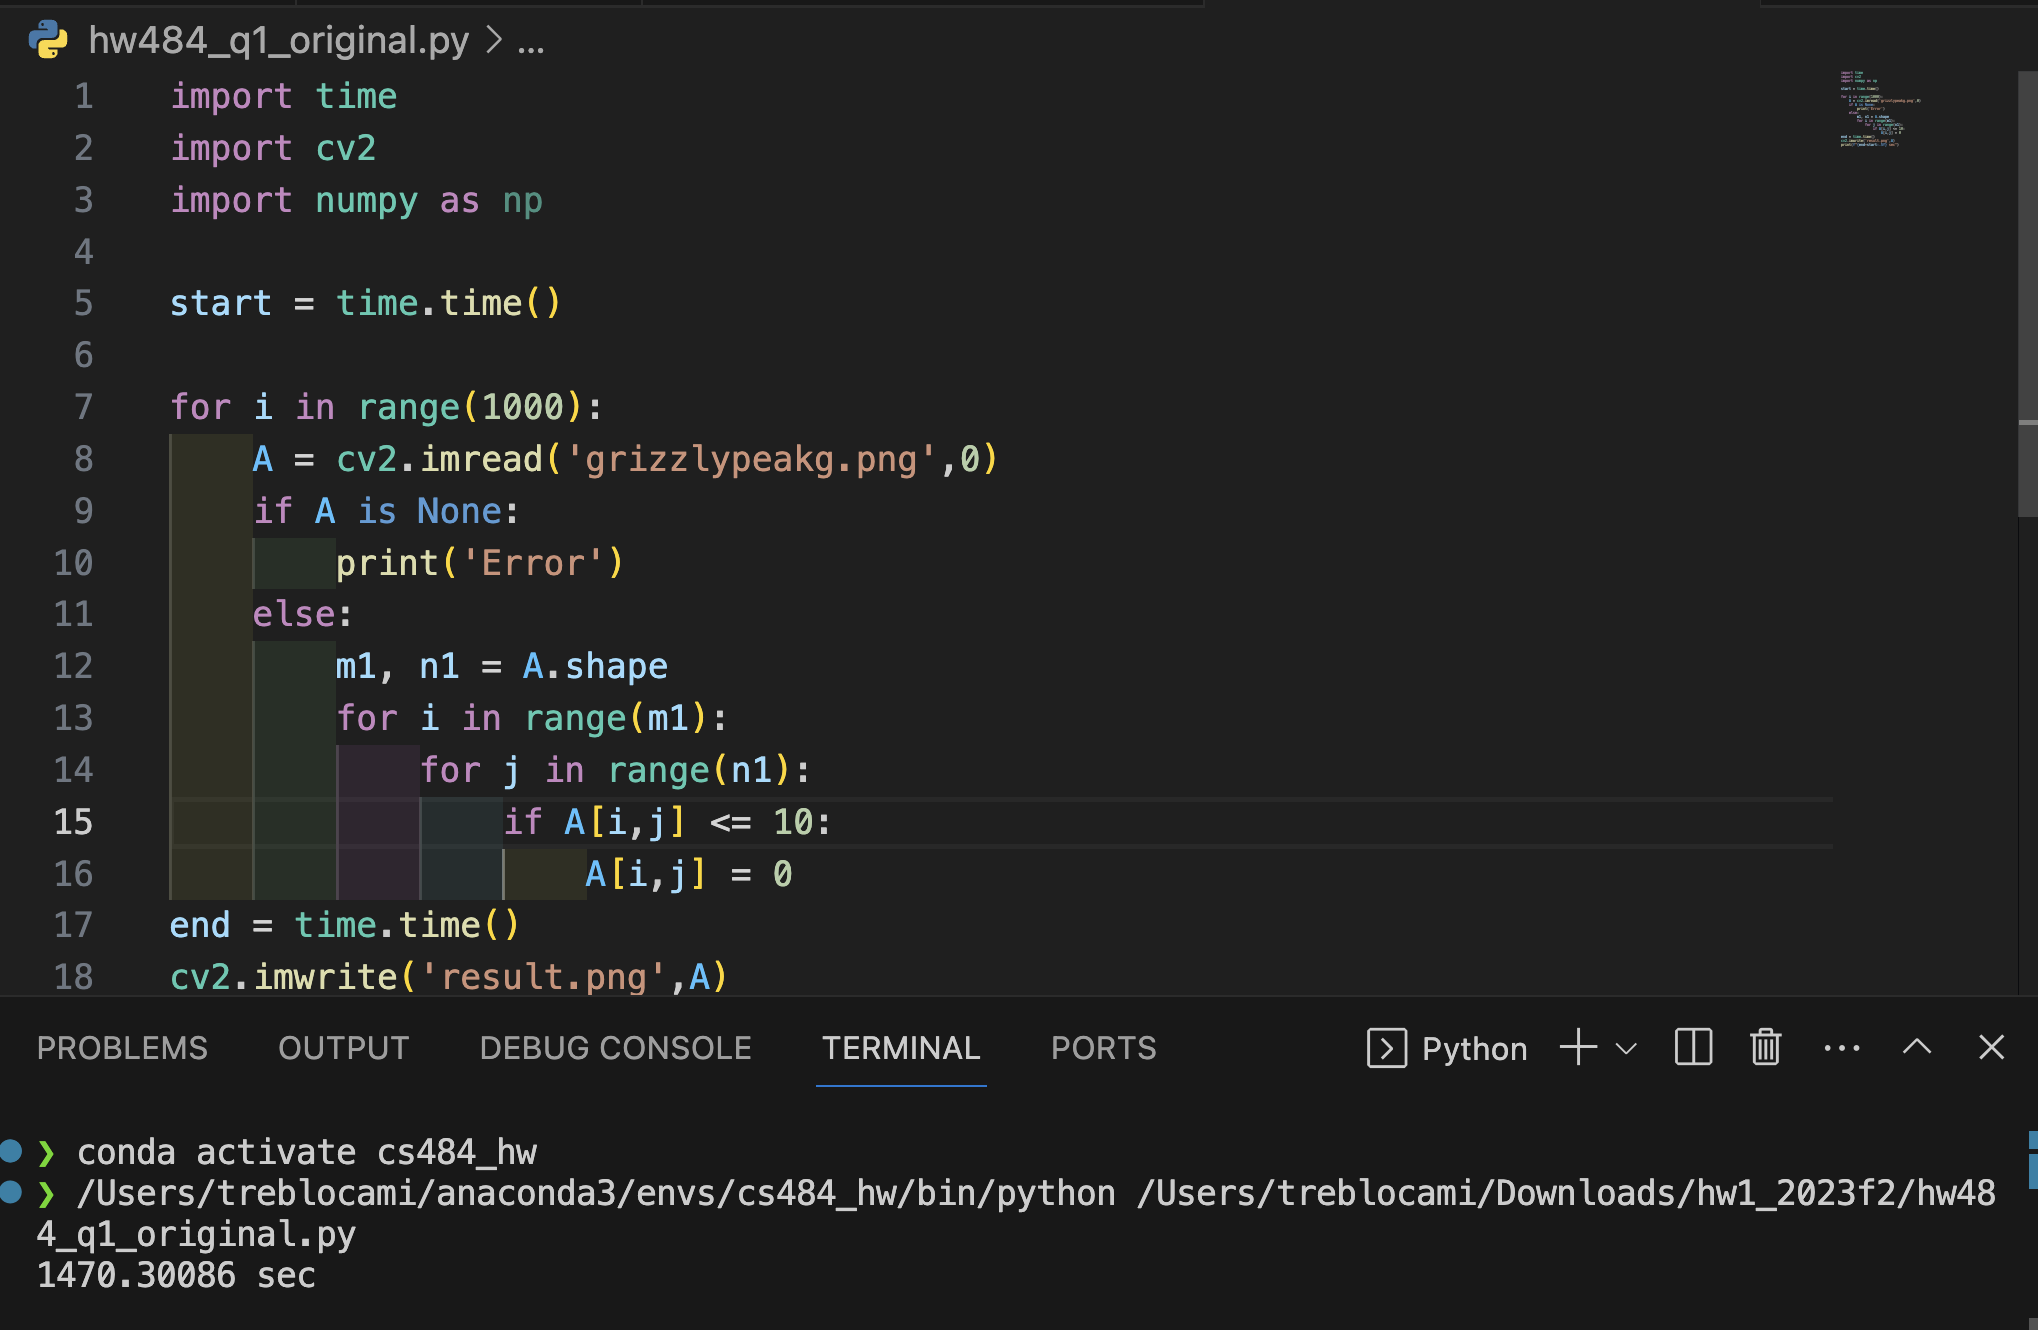
\includegraphics[width=9cm]{q1_original_execution.png}}
\caption{Execution Time of Original Code of Question 1}
\end{figure}

\begin{figure}
\centerline{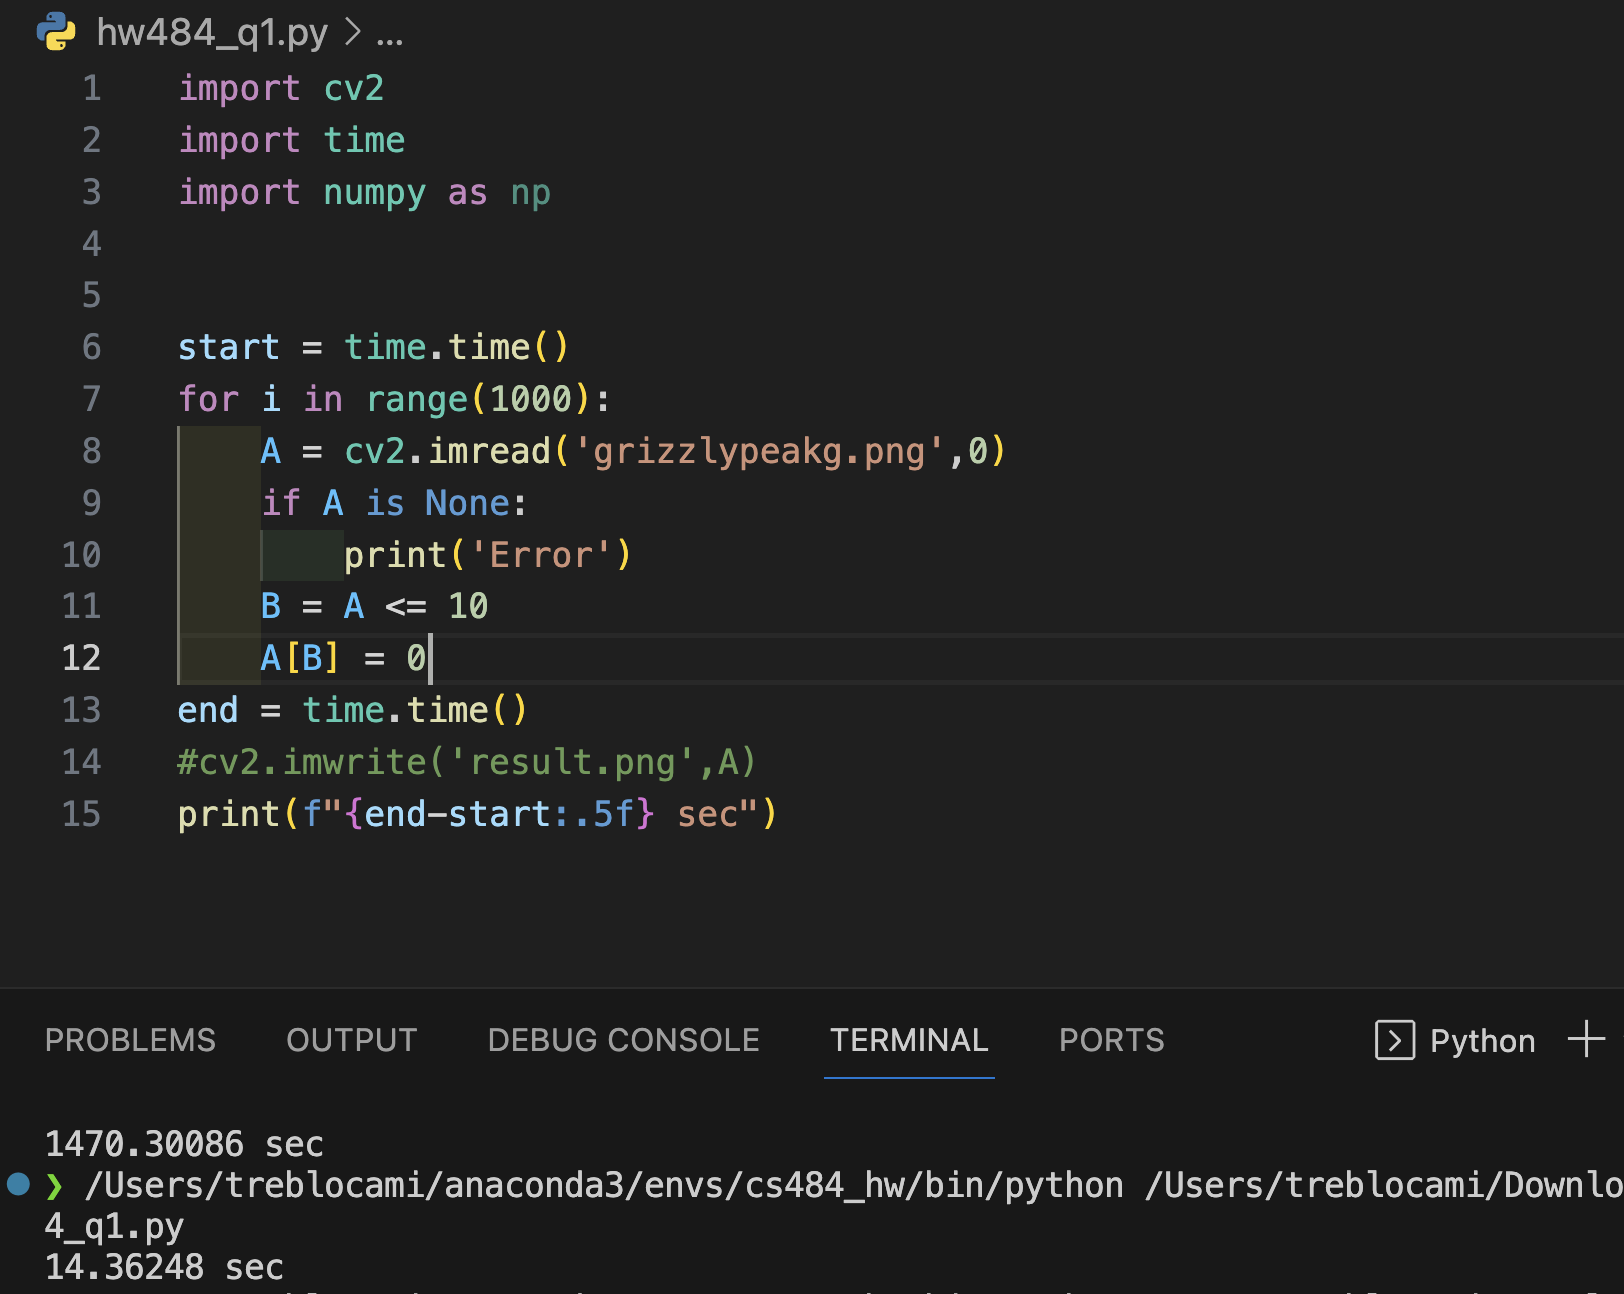
\includegraphics[width=9cm]{q1_execution.png}}
\caption{Execution Time of New Code of Question 1}
\end{figure}

\begin{figure}
\centerline{\includegraphics[width=4cm]{hw2_result.png}}
\caption{Result of New Code of Question 2}
\end{figure}
\end{document}
